\documentclass[12pt, a4paper]{article}
\RequirePackage[hmargin=2cm,vmargin=2cm]{geometry}

\usepackage[T1]{fontenc}
\usepackage{lmodern}
\usepackage{amssymb,amsmath}
\usepackage{authblk} % allows for better author affiliations

% Fancy HEADER
\usepackage{fancyhdr}
\pagestyle{fancy}
\pagenumbering{arabic}
\lhead{\itshape{\nouppercase{\leftmark}}}
\chead{}
\rhead{\thepage}
%\lfoot{v }
\cfoot{}
%\rfoot{\thepage}

% allows for numbered referencing, as refquired by ecol letters
\usepackage{etoolbox}
\newbool{MyRefNumbers}
\booltrue{MyRefNumbers} % comment to remove numbers in reference list

\usepackage{natbib}
\bibliographystyle{ecol_let}
\setcitestyle{authoryear,open={(},close={)}}

\usepackage{graphicx}
% We will generate all images so they have a width \maxwidth. This means
% that they will get their normal width if they fit onto the page, but
% are scaled down if they would overflow the margins.
\makeatletter
\def\maxwidth{\ifdim\Gin@nat@width>\linewidth\linewidth
\else\Gin@nat@width\fi}
\makeatother

\let\Oldincludegraphics\includegraphics
\renewcommand{\includegraphics}[1]{\Oldincludegraphics[width=\maxwidth]{#1}}

\usepackage[rgb,dvipsnames]{xcolor}
\definecolor{grey}{rgb}{0.5, 0.5, 0.5}

\usepackage[setpagesize=false, % page size defined by xetex
              unicode=false, % unicode breaks when used with xetex
              xetex]{hyperref}
\hypersetup{breaklinks=true,
            bookmarks=true,
            pdfauthor={},
            pdftitle={Untangling the link between traits, size and growth rate in plants},
            colorlinks=true,
            citecolor=black,
            urlcolor=grey,
            linkcolor=grey}
\setlength{\parindent}{0pt}
\setlength{\parskip}{6pt plus 2pt minus 1pt}
\setlength{\emergencystretch}{3em}  % prevent overfull lines

\title{\LARGE Untangling the link between traits, size and growth rate in plants}

\author[1]{Daniel S. Falster}
\author[1]{Richard G. FitzJohn}
\author[2]{Joe Wright}

\affil[1]{{\footnotesize Biological Sciences, Macquarie University, North Ryde, NSW 2109, Australia}}
\affil[2]{{\footnotesize Center for Tropical Forest Science, Smithsonian Tropical Research Institute, Panama, Republic of Panama}}
\renewcommand\Authands{ and }
\date{\vspace{-3em}}

\begin{document}

\maketitle
\thispagestyle{empty} % avoid header and footer on first page. Put after \maketitile, if using that

\section*{Abstract}\label{abstract}

\section*{Introduction}\label{introduction}

Functional traits are thought to capture core differences in the strategies
plants use to generate and invest surplus energy
\citep{wright_world-2004, chave-2009, westoby-2002}.
Although most plants have the same basic construction, physiological function
and resource requirements, species differ considerably from one another in
rates of carbon, nitrogen and water uptake, growth, mortality and seed
production. Some of these functional differences have been linked to
underlying variation in relatively simple physiological traits, such as leaf
mass per area (LMA), wood density (WD), leaf nitrogen per area, vessel
diameter,  and seed size  \citep{wright_world-2004,chave-2009}.
These traits are easily measured across diverse species, and variation between
species is large compared to variation within species. Data for some traits
now exists for up to 10\% of the world's 250000 plant species
\citep{cornwell-2014}. During the last decade, the idea has taken
hold that the growth strategy and ecology of a plant species might usefully be
characterised simply by knowing its traits.

While the influence of plant traits on elements of plant physiological
function is increasingly understood, attempts at using traits to understand
demographic rates have only met with mixed success
\citep{wright-2010, poorter-2008}. In seedlings, the trait LMA
-- a central part of the leaf economics spectrum
\citep{wright_world-2004} --is tightly related to plant relative growth
rate in mass \citep{lambers-1992, wright_cross-2000}. LMA and
its correlate leaf lifespan have also been linked to height growth rate for
small seedlings and saplings \citep{reich-1992, poorter-2006}. These
early successes prompted researchers to search for similar relationships in
large plants. However, the results showed that in trees LMA was not correlated
with diameter growth rate  \citep{wright-2010, poorter-2008,
herault-2011}. Meanwhile, other traits such as wood density showed
strong relationships to growth in large plants \citep{wright-2010},
but only weak relationships in seedlings  \citep{castro-diez-1998}. Thus
far, most trait growth relationships have been quantified for one or few
traits and at a single life- stage. Yet the picture is emerging is that the
link between traits and growth may be modified by plant size
\citep{ruger-2012}; a finding that challenges the wide-spread
assumption that particular ends of the trait spectrum translate directly into
faster or slower growth.

The challenge of interpreting diverse empirical results linking  -- or not --
traits to growth rate would clearly be easier with clear expectations on what
signal one should expect, given current understandings of how traits influence
plant function. Generating these expectations is a primary, yet perhaps under-
appreciated, role for theory \citep{kokko-2007}. Current empirical
results suggest the effect of traits on growth changes with size and possibly
also light environment, yet current theory says little about how such
relationships might come about. A widely-used model shows that for seedlings,
mass-based relative growth rate is linearly and negatively related to LMA
\citep{lambers-1992, cornelissen-1996,
wright_cross-2000}. An extension of the model suggests a similar
relationship may hold at larger sizes \citep{enquist-2007}. But as
described above, this prediction is not supported by empirical results.
Meanwhile, theoretical predictions on how other traits should influence growth
are largely absent.

A further problem with existing theory is that the effects of traits are all
realised via influences on mass production\citep{enquist-2007},
whereas the effect of traits such as LMA, WD, and Hmax is via the quality of
tissue construction, or the amount of mass allocated to different tissues
\citep{falster-2011}. There are in fact two problems with theory
focussed solely on mass production. The first is that measuring mass
production is only practical for small plants that can be easily harvested.
For larger plants, growth is more often measured either as diameter or height
growth. For example, the CTFS monitors diameter growth in 49 large permanent
plots across forests worldwide \citep{anderson_teixeira_ctfs-2014},
while forestry agencies around the world have likewise recorded data across
large tracts of forest \citep{purves-2008}. The second problem is
that, as we outline further below, because mass production is only one
component of plant growth; theory focussing solely on mass production will
therefore always be limited.

In this paper we provide a mechanistic framework for describing the potential
effect of traits on growth throughout a plant's life-cycle, linking to
commonly used metrics such as height and diameter growth. To help motivate our
study we re-analyse demographic and trait data from an earlier study
\citep{wright-2010}, to show 1) that the link between traits and
growth is stronger than previously thought, 2) that the influence of three
prominent traits on growth rate is moderated by plant size, and 3) that the
impact of size on the nature of relationships varies among traits (see also
\citet{ruger-2012}. We then show how these results align with new
set of theoretical predictions. Moreover, we show how traits moderate plant
responses to light environment and also determine shade tolerance, supporting
diverse empirical results \citep{ruger-2012, poorter-2006}. By
disentangling the effects of plant size, light environment and traits on
growth rates, we hope to provide a solid theoretical foundation for trait
ecology and thus provide a platform for understanding growth across diverse
species around the world.

\subsection*{Empirical motivation}\label{fresh-empirical-motivation}

To help illustrate the empirical patterns, we begin with a fresh analysis of
growth dynamics in the long-term plot at Barro Colorado Island in Panama,
where the growth rates for over 100 species have been recorded over the last
30 years. Data from a long term plot \citep{condit-2012} are combined
with results of experiment on seedlings \citep{kitajima-2013}, to better understand
size-related patterns of growth. A prior analysis by
\citet{wright-2010} found a moderate effect of wood density on
growth rate, but almost no effect of LMA, and only a weak effect of HMAX. More recently,
\citet{ruger-2012} showed

\begin{itemize}
\itemsep1pt\parskip0pt\parsep0pt
\item
  Effect of lma stronger than previously thought,
\item
  Bridges from seedling studies to adults
\end{itemize}

Results stronger than previously reported.

\section*{Materials and Methods}\label{materials-and-methods}

\subsection*{Conceptual framework}\label{conceptual-framework}

Builds on 2011 paper - highlight what's new from there.

Decomposition of diameter and height growth

Functional-balance Model of growth

\begin{itemize}
\itemsep1pt\parskip0pt\parsep0pt
\item
  four key assumptions.
\item
  simple linear functions non-critical for results of this paper,
\item
  explore using an example model, but any model with basic size effects
  will display same behaviour

  \begin{itemize}
  \itemsep1pt\parskip0pt\parsep0pt
  \item
    details about our model ()
  \item
    show argument hold intuitively
  \end{itemize}
\end{itemize}

Embedding trait-related trade-offs

\begin{itemize}
\itemsep1pt\parskip0pt\parsep0pt
\item
  use table with arrows to
\end{itemize}

Connection to earlier work

\begin{itemize}
\itemsep1pt\parskip0pt\parsep0pt
\item
  generalised version
\item
  present old model as dp/dt so consistent with ours
\end{itemize}

\subsection*{Analysis}\label{analysis}

\subsection*{Growth data}\label{growth-data}

\section*{Results}\label{results}

\subsection*{Changes in growth rate with
size}\label{changes-in-growth-rate-with-size}

\subsection*{How traits influence growth
rate}\label{how-traits-influence-growth-rate}

\subsubsection*{LMA}\label{lma}

\subsubsection*{Wood density}\label{wood-density}

\subsubsection*{HMax}\label{hmax}

\section*{Discussion}\label{discussion}

\begin{itemize}
\itemsep1pt\parskip0pt\parsep0pt
\item
  mechanistic model of height and dbh growth which accounts for effects
  of size, light environment and traits

  \begin{itemize}
  \itemsep1pt\parskip0pt\parsep0pt
  \item
    need to account for size long recognized, but not straightforward
  \item
    look at growth in wide range of measures: mass, height, dbh
  \end{itemize}
\item
  Compared to previous work, shows effects of traits more about
  allocation than mass production
\end{itemize}

\subsection*{Tree growth is more than just
photosynthesis}\label{tree-growth-is-more-than-just-photosynthesis}

Recently realisation that allocation and turnover major areas of
uncertainty

Model reconciles idea that traits can have negative impact on carbon
budget, but still have positive influence on growth rates

\begin{itemize}
\itemsep1pt\parskip0pt\parsep0pt
\item
  Enquist 2007: sla and wd increase mass-production, where as in our
  theory effects on mass production are negative. (also contradicts
  earlier model from Enquist 1999, where argued wood density had no
  effect on mass production)
\end{itemize}

Assumes low lma and wd used to reduce costs of building leaf and stem,
ie. total leaf area and stem corss section remains same. In this way
differs to assumptions of recent work by anten\_role\_2010,
larjavaara\_rethinking\_2010.

Model is realisation of several ideas that have been around for some
time.

Plasticity in trait values predicted from model:

@Osazuwa-Peters-2014 - indreases in WD through ontogeny.

\subsection*{Towards a global model of tree
growth}\label{towards-a-global-model-of-tree-growth}

Key patterns explained

Data challenges

Reproductive allocation

\subsection*{Detecting trait signals in
data}\label{detecting-trait-signals-in-data}

Need more than simply look for correlation with mean growth rate

\begin{itemize}
\itemsep1pt\parskip0pt\parsep0pt
\item
  understand influences of size on trait of interest
\item
  traits define potential growth rate --\textgreater{} how to extract
  this
\item
  ideally start to use mechanistic models
\end{itemize}

\subsection*{Implications for trait-based
approaches}\label{implications-for-trait-based-approaches}

How do comparative people interpret sla now - beyond fast slow.

Think about traits as defining potential trajectory, rather than making
species fast or slow growing per se.

Selection on traits in different parts of lifecycle

Trait plasticity - can explain, no clear advantage of low lma at large
sizes

Framework for generalising about effect of traits

\section*{Conclusion}\label{conclusion}

\newpage

\section*{Tables}\label{tables}

\textbf{Table 1 - Key equations of growth model}

\begin{itemize}
\itemsep1pt\parskip0pt\parsep0pt
\item
  key parameters of model
\end{itemize}

\textbf{Table 2 - effect of traits on demography}

\begin{itemize}
\itemsep1pt\parskip0pt\parsep0pt
\item
  combines previous tables 1 \& 2
\end{itemize}


\newpage

\section*{Figures}\label{figures}

\begin{figure}[htbp]
\centering
\includegraphics{figures/BCI_data2.pdf}
\caption{\textbf{The relationship between traits and potential growth
rate varies with plant size.} For XXX species from tropical rain forest
in Panama, we estimated the potential growth rate of individual's in
each species at a series of diameters \(D\), indicated along right hand
side. The size of circles in each panel indicates the number of data
points used to estimate potential growth rate. Traits values were
calculated from representative individuals in each species.
\label{f-BCI}}
\end{figure}

\newpage

\begin{figure}[htbp]
\centering
\includegraphics{figures/SI_size_dhdt.pdf}
\caption{\textbf{Conceptual framework for understanding size-dependent
changes in growth rate.} \label{f-conceptual}}
\end{figure}

\newpage

\begin{figure}[htbp]
\centering
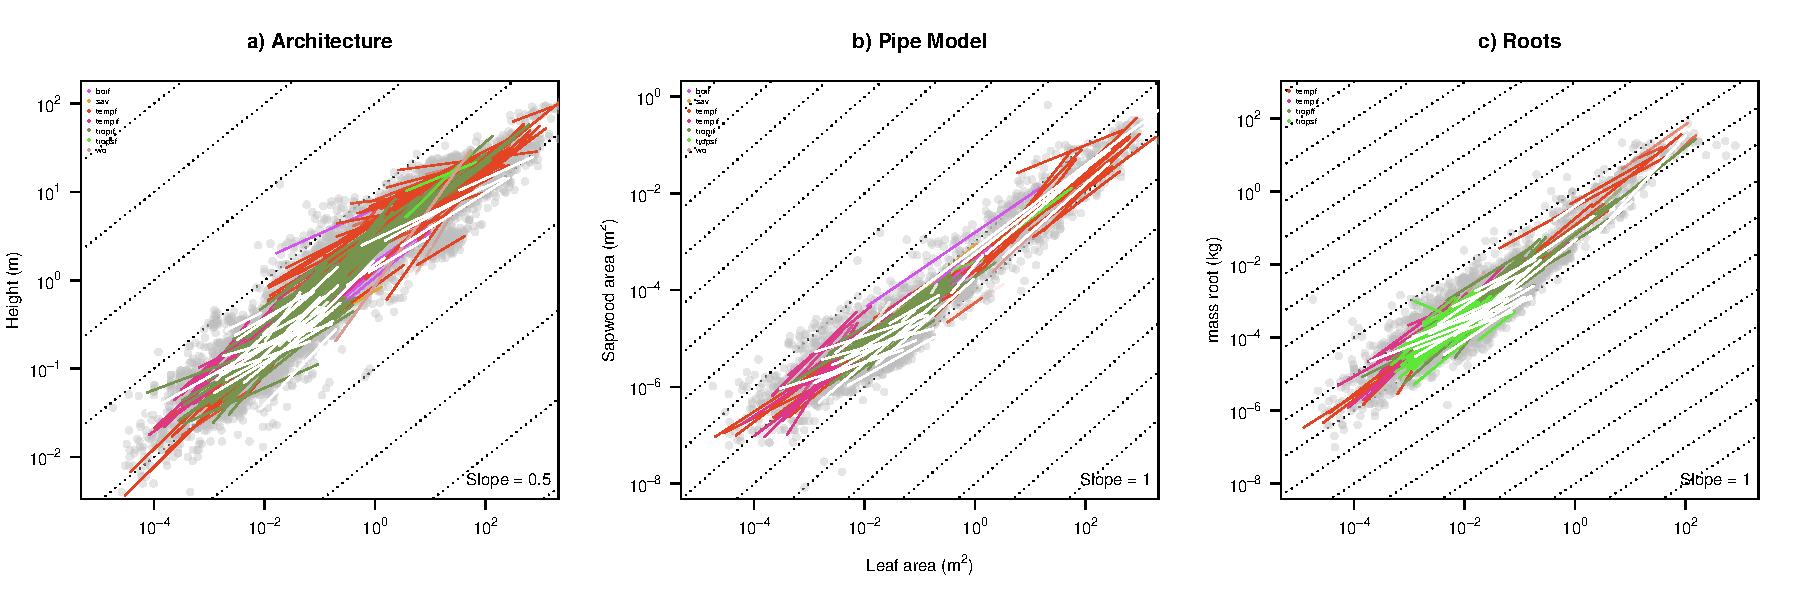
\includegraphics{figs/allometry.pdf}
\caption{\textbf{Key assumptions of a functional balance and trait
trade-offs model, evaluated using global dataset.} We used the biomass and
allometry database to evaluate model assumptions about \textbf{a,}
scaling of leaf area with plant height, \textbf{b} Scaling of sapwood
area with leaf area, and \textbf{c} scaling of root mass with leaf area.
Each dot is a single plant. Lines show standardised major axis lines
fitted to data from each site, with intensity of shading adjusted
according to strength of the relationship. Colours indicate vegetation
type. Dashed black lines show values expected under functional-balance
assumption (see Supplementary text for details). \label{f-assumptions}}
\end{figure}

\newpage

\begin{figure}[htbp]
\centering
\includegraphics{figures/growth_light.pdf}
\caption{\textbf{Traits moderate the responsiveness of growth to changes
in light environment.} Panels show predicted relationship between
specific trait and diameter growth rate, for a plant of specified
diameter and under a range of shading environments.
\label{f-growth_light}}
\end{figure}

\newpage

\begin{figure}[htbp]
\centering
\includegraphics{figures/max_leaf_above.pdf}
\caption{\textbf{The effect of traits on growth changes with size and
light environment.} Traits moderate the responsiveness of growth to changes in light
environmentThis figure needs to show more of key result with respect to to size.
Possibly separate figure. \label{f-shifts}}
\end{figure}

\newpage

\begin{figure}[htbp]
\centering
\includegraphics{figures/max_leaf_above.pdf}
\caption{\textbf{Low construction cost leads to shade intolerance,
because of costs of high turnover.} Panels show effect of traits on
maximum amount of shading that can be endured before net production (eq.
\ref{eq:dPdt}) reaches zero. Lines indicate relationship for plants of a
given height. \label{f-wplcp}}
\end{figure}

\newpage

\bibliography{references}
\end{document}